\documentclass{exam}

%------------------------ packages ------------------------%
\usepackage{amsmath,amsfonts,amsthm,amssymb,amsopn,bm}
\usepackage{pythontex}
\usepackage{fullpage}
\usepackage{graphicx}
\usepackage{fullpage}
\usepackage[paper=letterpaper,margin=1in,includeheadfoot,footskip=0.25in,headsep=0.25in]{geometry}
\usepackage{url}
\usepackage[usenames,dvipsnames]{color}
\usepackage[pdfborder={0 0 1},colorlinks=true,citecolor=black,plainpages=false]{hyperref}
%\usepackage{fancyhdr}
\usepackage{multirow}
\usepackage[english]{babel}
\usepackage{pdfpages,bbm}
\usepackage{enumitem}
\usepackage{todonotes}
\usepackage{tikz}
\usetikzlibrary{arrows,automata}


%------------------------ math ------------------------%
\newcommand{\R}{\mathbb{R}} % real domain
\newcommand{\Rset}{\mathbb{R}} % real domain
\newcommand{\argmin}{\operatorname{argmin}}
\newcommand{\argmax}{\operatorname{argmax}}
\newcommand{\xv}{\mathbf{x}}
\newcommand{\av}{\mathbf{a}}
\newcommand{\bv}{\mathbf{b}}
\newcommand{\yv}{\mathbf{y}}
\newcommand{\wv}{\mathbf{w}}
\newcommand{\uv}{\mathbf{u}}
\newcommand{\zv}{\mathbf{z}}
\newcommand{\Xv}{\mathbf{X}}
\newcommand{\W}{\mathbf{W}}
\newcommand{\K}{\mathbf{K}}
\newcommand{\M}{\mathbf{M}}
\newcommand{\C}{\mathbf{C}}
\newcommand{\B}{\mathbf{B}}
\newcommand{\X}{\mathbf{X}}
\newcommand{\I}{\mathbf{I}}
\newcommand{\Proj}{\mathbf{P}}
\newcommand{\Y}{\mathbf{Y}}
\newcommand{\U}{\mathbf{U}}
\renewcommand{\L}{\mathbf{L}}
\newcommand{\y}{\mathbf{y}}
\newcommand{\x}{\mathbf{x}}
\newcommand{\w}{\mathbf{w}}
\newcommand{\mD}{\mathbf{D}}
\newcommand{\A}{\mathbf{A}}
\newcommand{\zero}{\mathbf{0}}
\newcommand{\norm}[1]{\left\lVert#1\right\rVert}
\DeclareMathOperator{\rank}{rank}
\newcommand{\E}{\mathbb{E}}


%------------------------ exam class macros ------------------------%
\checkboxchar{$\Box$}
% \renewcommand{\questionshook}{%
%     \setlength{\leftmargin}{10pt}%
%     \setlength{\labelwidth}{-\labelsep}%
% }
\renewcommand{\checkboxeshook}{
  \settowidth{\leftmargin}{W.}
  \labelwidth\leftmargin\advance\labelwidth-\labelsep
}

\newcommand{\grade}[1]{\small\textcolor{magenta}{\emph{[#1 points]}} \normalsize}

\begin{document}

\title{Homework 5 Written Assignment}
\author{\Large \bf 10-605/10-805: Machine Learning with Large Datasets}
\date{{\bf Due Thursday, November \Large{November 19}th at 1:30:00 PM Eastern Time}}
\maketitle

\paragraph{Instructions:} Submit your solutions via Gradescope, \textit{with your solution to each subproblem on a separate page}, i.e., following the template below.  Note that Homework 5 consists of two parts: this written assignment, and a programming assignment. The written part is worth \textbf{50\%} of your total HW5 grade. The programming part makes up the remaining 50\%.

\paragraph{Submitting via Gradescope:} When submitting on Gradescope, you must assign pages to each question correctly (it
prompts you to do this after submitting your work). This significantly streamlines the
grading process for the course staff.  Failure to do this may result in a score of 0 for any questions
that you didn't correctly assign pages to. It is also your responsibility to make sure that your scan/submission is legible so that we can grade it.

\paragraph{Collaboration:}  While you may talk with others about the homework, you must each turn in your own solution and it should be your own work. \text{Please list the names of any collaborators below.}

\paragraph{Collaborators:}


\newpage
\noindent As we consider more hyperparameters, the space we search over to find good hyperparameter configurations grows very quickly. In the first two questions, we will explore just how quickly this space grows.

\section{Curse of Dimensionality (\Large{12} pts)}

We define the $\epsilon$-cover of a search space $S$ as a subset $E \subset S$:
\[ 
    E = \{x \in \mathbb{R}^n\ |\ \forall y \in S,\,\exists x\ s.t.\ \|y-x\|_\infty \leq \epsilon\}
\]
In words, every coordinate of every point in our search space $S$ is within $\epsilon$ of a point in our set $E$. %(Note that the generalization of this works for any pseudometric distance d between any two points).
The $\epsilon$-covering number is the size of the smallest such set that provides an $\epsilon$-cover of $S$.
\[
    N(\epsilon, S) = \min_E \{|E|  : E \textrm{ is an } \epsilon\textrm{-cover of } S\}
\]
Let's work through a concrete example to make the concept clearer: let's say we want to tune the learning rate for gradient descent on a logistic regression model by considering learning rates in the range of $[1,2]$. We want to have $\epsilon=.05$-coverage of our search space $S = [1,2]$. Then $E = \{1.05, 1.15, 1.25, 1.35, 1.45, 1.55, 1.65, 1.75, 1.85, 1.95\}$. We see that any point in $[1,2]$ is within $0.05$ of a point in $E$. So $E$ provides $\epsilon$-coverage of $S$. The $\epsilon$-covering number is 10. The questions below will ask you to generalize this idea.
\begin{enumerate}[label=(\alph*)]
    \item \grade{4} Find the size of a set needed to provide $\epsilon$-coverage ($\epsilon$-covering number) of $S = [0,1]\times[0,2]$, the Cartesian product of two intervals. Note that we want this to hold for a generic $\epsilon$.
    
    \vspace{2in}
    \item \grade{8} Find the $\epsilon$-covering number of $S = [a_1, b_1] \times \ldots \times [a_d, b_d]$, the Cartesian product of $d$ arbitrary closed intervals. On what order does this grow with respect to the dimension $d$ and interval lengths (i.e., with the volume of this space)?
\end{enumerate}

\clearpage
\section{Grid versus Random Search (\Large{12} pts)}
There are two basic strategies commonly employed in hyperparameter search: grid search and random search. Grid search is defined as choosing an independent set of values to try for each hyperparameter and the configurations are the Cartesian product of these sets. Random search chooses a random value for each hyperparameter at each configuration. Imagine we are in the (extreme) case where we have $d$ hyperparameters all in the range $[0,1]$, but only \emph{one} ($h_1$) of them has any impact on the model, while the rest have \emph{no} effect on model performance. 
\begin{enumerate}[label=(\alph*)]
    \item \grade{4} Imagine that we consider $q$ hyperparameter configurations, which are enough to provide $\epsilon$-coverage for grid search. How many unique models will we train? What is this as a percent of the total number of configurations?
    
    \vspace{1.5in}
    \item \grade{4} Alternatively, if we consider $q$ random configurations as part of random search, then what percent of the configurations will cause a change to the model?  Why?
    
    \vspace{1.5in}
    \item \grade{4} Now we change our point of view; instead of desiring $\epsilon$-coverage, we have a fixed budget of $B \ll |S|$ configurations to try. Which search strategy should we employ? Why?
    
    
\end{enumerate}


\clearpage
\section{Uniform Allocation versus Early Stopping (\Large{26} pts)}

Consider two configurations, and imagine we plot validation error as a function of number of iterations (or resources).  This validation error is noisy since it's based on partially trained models. However, let's assume we know that these models eventually converge to some fixed validation errors $\nu_1$ and $\nu_2$, which implies that there exists some envelope of uncertainty bounding this noise. For simplicity, imagine we have the same envelope of uncertainty for both configurations, $\gamma_k$, which is a function of the $k$, the number of iterations run. Figure~\ref{fig:bands} below will aid you in visualizing what we are looking for.

\begin{figure}[bh]
    \centering
    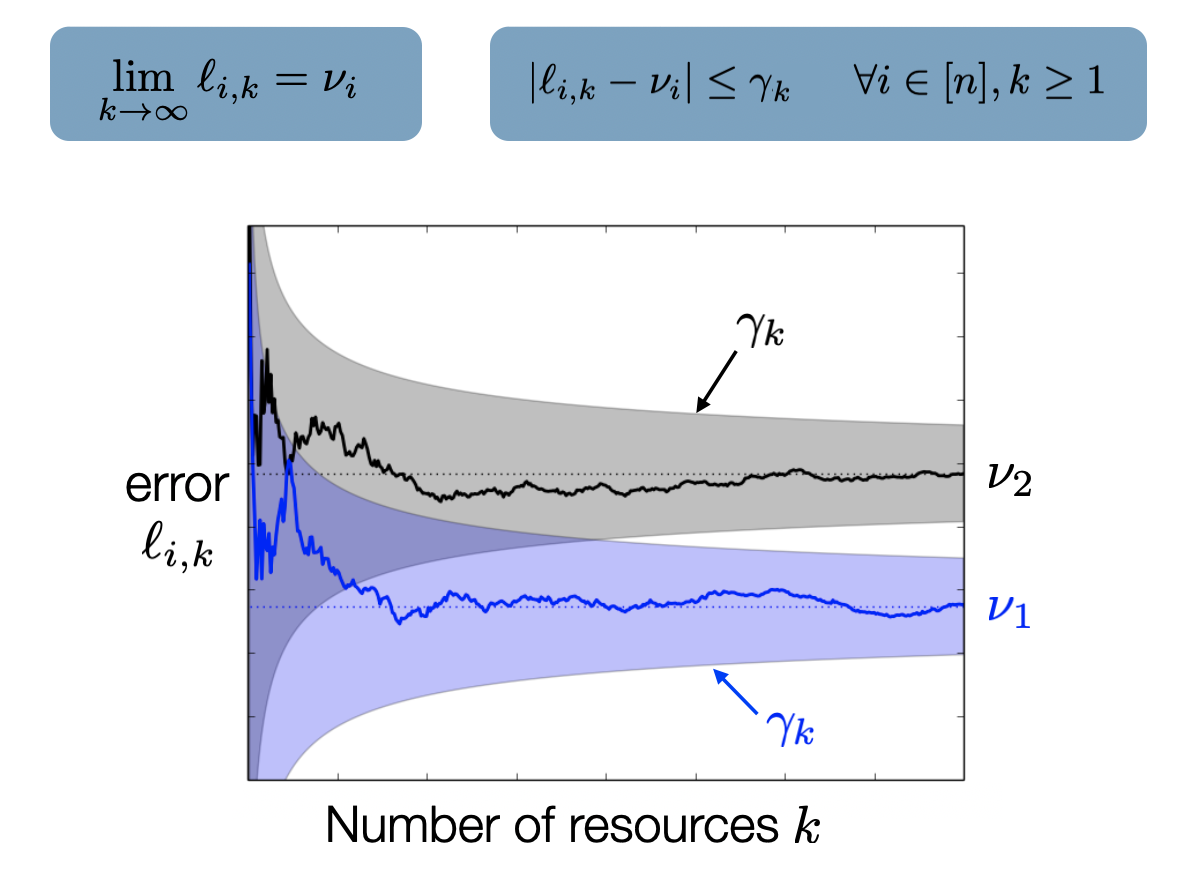
\includegraphics[width=.5\textwidth]{hw5/bands_of_uncertainty.png}
    \caption{A visualization of the envelopes of uncertainty around the true convergent validation errors at each training iteration.}
    \label{fig:bands}
\end{figure}

\begin{enumerate}[label=(\alph*)]

\item \grade{5} What are the possible values for configuration 1 validation error after $k=1$ iteration, expressed in terms of $\nu_1$ and $\gamma_1$?
    

\vspace{.5in}

\item \grade{5} Now imagine we were given access to this envelope of uncertainty. At what point could we, with certainty, know that configuration 1 is better than configuration 2? Can you express this mathematically as a function of the given $\gamma_k$, $\nu_2$ and $\nu_1$? Show your work. 
    
\vspace{0in}
\end{enumerate}


\clearpage
 Next, imagine the we have $N$ configurations we're considering (with their quality ordered by configuration number, i.e., configuration 1 is the best, configuration 2 is second best, etc.), all of which are governed by the same envelope of uncertainty. Our goal is to find an efficient allocation of resources across these N configurations, i.e., to choose how many iterations to run each configuration for such that we identity the best configuration with the fewest number of total iterations. 

\begin{enumerate}[label=(\alph*)]
\setcounter{enumi}{2}
    \item \grade{8} Consider a uniform allocation strategy, as is done with vanilla random search, in which we are required to allocate the same number of iterations to all configurations.  What is our required total budget in order to, with certainty, be able to identify that configuration 1 is the best?  Please characterize this total budget as a function of $\nu_i$ and $\gamma$.
    
    \vspace{1in}

\clearpage

\begin{figure}[bh]
    \centering
    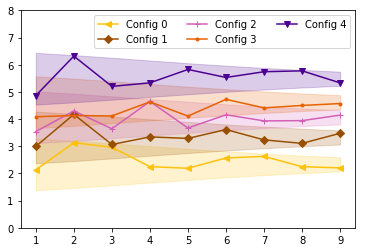
\includegraphics[width=.6\textwidth]{hw5/adaptive_example.png}
    \caption{Validation loss as a function of iteration number for five configurations.  Note that the shaded regions are the associated regions of uncertainty.}
    \label{fig:adaptive_example}
\end{figure}    
    
    \item \grade{8}  Now imagine we are in the situation of  Figure~\ref{fig:adaptive_example}. We run iterations one at a time for each configuration we haven't ruled out as being best. At each iteration, we adaptively choose whether to continue running that configuration or not. How many configuration-iterations will we have run? This will be lower-bounded by 5 (running them all for one iteration and stopping) and 45 (running all configurations for all 9 iterations of the experiment). How does this adaptive allocation approach compare to the uniform allocation strategy previously discussed?  Please fill out the table below.

    Note: The simple answer is `0', we already know $\nu_1,\dots,\nu_5$. We are \emph{not} looking for this answer. Instead, we are considering the artificial exercise of only using $\nu_i$ to center our $\gamma_k$, and to make decisions based on these centered $\gamma_k$. 
    
    Note: We will accept some minor variations to our expected final answers given that slight visual ambiguity of the shaded  regions of uncertainty in Figure~\ref{fig:adaptive_example}.
    
\renewcommand{\arraystretch}{2}
   \begin{table}[ht]
        \begin{tabular}{|c|c|c|}\hline
        \textbf{Configuration} & \textbf{Iterations with Uniform Allocation} & \textbf{Iterations with Adaptive Allocation}  \\ \hline\hline
        0 & & \\ \hline
        1 & & \\ \hline
        2 & & \\ \hline
        3 & & \\ \hline
        4 & & \\ \hline
        sum & & \\ \hline
    \end{tabular}
    \end{table}

\end{enumerate}


\end{document}